%============================================================
%  Capitolo 13 – Diffusion Models
%============================================================
\chapter{Diffusion Models}
\label{ch:diffusion}

I \textbf{modelli di diffusione} (\emph{diffusion models}) rappresentano
la classe di modelli generativi allo stato dell'arte per la sintesi di
immagini ad alta qualità. A differenza delle GAN (Cap.~\ref{ch:gans}),
che apprendono implicitamente la distribuzione dei dati attraverso un
gioco adversariale, i modelli di diffusione apprendono a \emph{invertire}
un processo stocastico di corruzione progressiva dei dati
\citep{bishop2024}. Il modello più noto che sfrutta questa architettura
è \textbf{Stable Diffusion}, un \emph{latent diffusion model} (LDM) che
sposta il processo di diffusione dallo spazio dei pixel a uno spazio
latente compresso, ottenendo un drastico miglioramento dell'efficienza
computazionale.

%------------------------------------------------------------
\section{Stable Diffusion: Architettura Generale}
\label{sec:sd-architecture}

Stable Diffusion è in grado di ricevere come input un \textbf{prompt
testuale} (text-to-image) oppure la combinazione di un testo e
un'immagine di riferimento (text\,+\,image), producendo in uscita
un'immagine sintetica coerente con le indicazioni fornite.

\subsection{Componenti Principali}
\label{subsec:sd-components}

L'architettura di Stable Diffusion è articolata in tre macro-componenti
che operano in sequenza:

\begin{description}
  \item[Text Encoder (CLIPText)] Converte il prompt testuale in una
        sequenza di embedding numerici. Riceve in ingresso fino a 77
        token e produce in uscita 77 vettori di embedding, ciascuno con
        768 dimensioni.
  \item[Image Information Creator (UNet + Scheduler)] È il nucleo del
        modello e il responsabile principale del miglioramento
        qualitativo rispetto ai modelli precedenti. Opera \emph{interamente
        nello spazio latente} e genera iterativamente le informazioni
        sull'immagine attraverso un numero configurabile di passi
        (tipicamente 50 o 100). La sua implementazione tecnica è basata
        su una rete \textbf{UNet} e un \textbf{algoritmo di scheduling}.
  \item[Image Decoder (Autoencoder Decoder)] Converte il tensore di
        informazioni latenti elaborato nella corrispondente immagine
        nello spazio dei pixel. Riceve in ingresso un tensore di
        dimensioni $(4, 64, 64)$ e produce un'immagine di dimensioni
        $(3, 512, 512)$, corrispondenti ai canali
        (rosso/verde/blu, larghezza, altezza).
\end{description}

\begin{figure}[H]
  \centering
  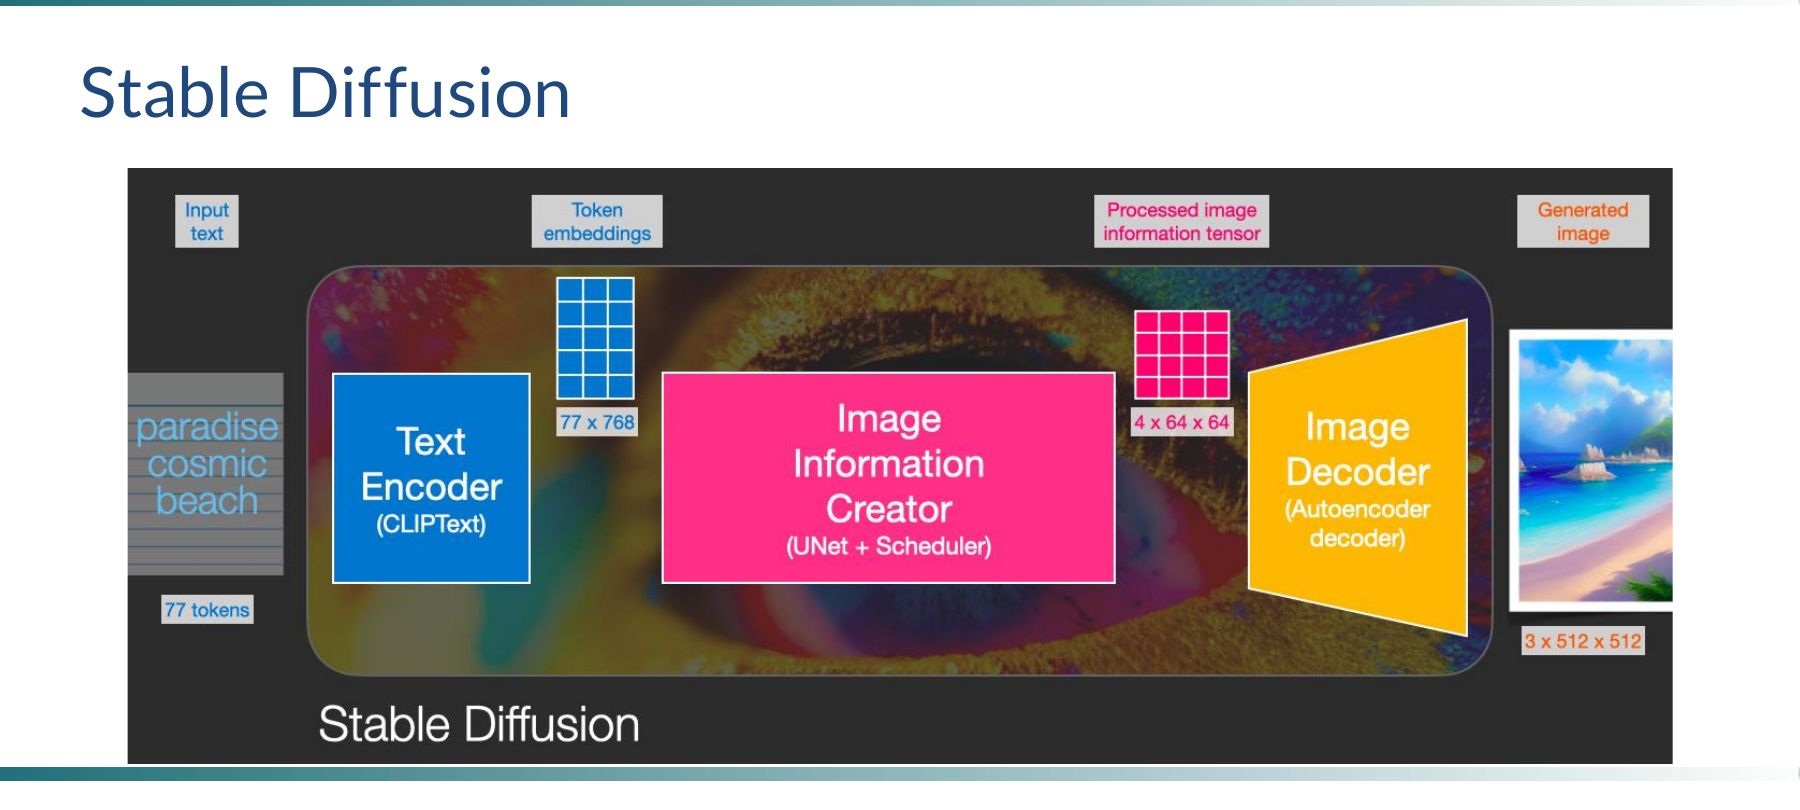
\includegraphics[width=0.92\linewidth]{figures/cf13_sd_full_pipeline.png}
  \caption{Architettura di Stable Diffusion. Il testo in ingresso
           viene prima codificato dal \emph{Text Encoder} (CLIPText)
           in 77 token embedding di dimensione 768. L'\emph{Image
           Information Creator} (UNet + Scheduler) opera nello spazio
           latente producendo un tensore $4\times64\times64$, che viene
           infine decodificato dall'\emph{Image Decoder} (autoencoder
           decoder) nell'immagine finale $3\times512\times512$.}
  \label{fig:sd_components}
\end{figure}

Il processo complessivo si divide in tre fasi numerate:
\begin{enumerate}
  \item Il \textbf{Text Encoder} converte i 77 token di input negli
        embedding testuali.
  \item L'\textbf{Image Information Creator} riceve gli embedding
        testuali e un tensore di rumore casuale, e li elabora
        attraverso la diffusione latente.
  \item L'\textbf{Image Decoder} traduce il tensore latente elaborato
        nell'immagine generata.
\end{enumerate}

%------------------------------------------------------------
\section{Il Processo di Diffusione}
\label{sec:diffusion-process}

\subsection{Forward Diffusion: Corruzione con Rumore}
\label{subsec:forward-diffusion}

Il \textbf{processo di diffusione in avanti} (\emph{forward diffusion})
consiste nel costruire il dataset di addestramento del predittore del
rumore. Dato un'immagine del dataset, si generano esempi di
addestramento secondo lo schema seguente:

\begin{enumerate}
  \item Si seleziona un'immagine dal dataset di addestramento.
  \item Si genera un campione di rumore casuale.
  \item Si seleziona una quantità di rumore da aggiungere.
  \item Si aggiunge il rumore all'immagine nella quantità stabilita.
\end{enumerate}

Poiché la quantità di rumore è controllabile con precisione, è possibile
creare decine di esempi di addestramento per ogni immagine, distribuendo
la corruzione su decine di passi discreti.

\subsection{Addestramento del Predittore del Rumore}
\label{subsec:noise-predictor-training}

Il dataset così costruito, in cui ogni esempio è composto da
(immagine corrotta, quantità di rumore aggiunta, campione di rumore
effettivo), viene utilizzato per addestrare un modello denominato
\textbf{Noise Predictor}, implementato come rete \textbf{UNet}.
Un singolo passo di addestramento comprende:

\begin{enumerate}
  \item Selezionare un esempio di addestramento dal dataset.
  \item Far predire alla UNet il campione di rumore contenuto
        nell'immagine.
  \item Calcolare la \emph{loss} confrontando la previsione con il
        rumore effettivo.
  \item Aggiornare i pesi del modello tramite backpropagation.
\end{enumerate}

\subsection{Reverse Diffusion: Rimozione Iterativa del Rumore}
\label{subsec:reverse-diffusion}

Una volta addestrato, il \emph{Noise Predictor} è in grado di stimare
il rumore contenuto in un'immagine rumorosa. La generazione di nuove
immagini sfrutta la \textbf{diffusione inversa} (\emph{reverse
diffusion}):

\begin{enumerate}
  \item Si genera un tensore completamente casuale (rumore puro).
  \item Il predittore del rumore stima il rumore presente.
  \item Il rumore stimato viene sottratto dal tensore corrente,
        ottenendo un'immagine leggermente de-rumorata.
  \item I passi 2 e 3 vengono ripetuti per un numero fissato di
        iterazioni di campionamento.
\end{enumerate}

Ripetendo questo processo, l'immagine ``emerge'' progressivamente dal
rumore. Se il dataset di addestramento era composto da immagini
esteticamente pregevoli (ad esempio LAION Aesthetics, su cui è stato
addestrato Stable Diffusion), l'immagine generata tenderà ad essere
anch'essa esteticamente pregevole. Il risultato finale dipende dunque
direttamente dalla natura del dataset di addestramento: un modello
addestrato su loghi produrrà loghi, uno addestrato su fotografie
produrrà fotografie.

\begin{figure}[H]
  \centering
  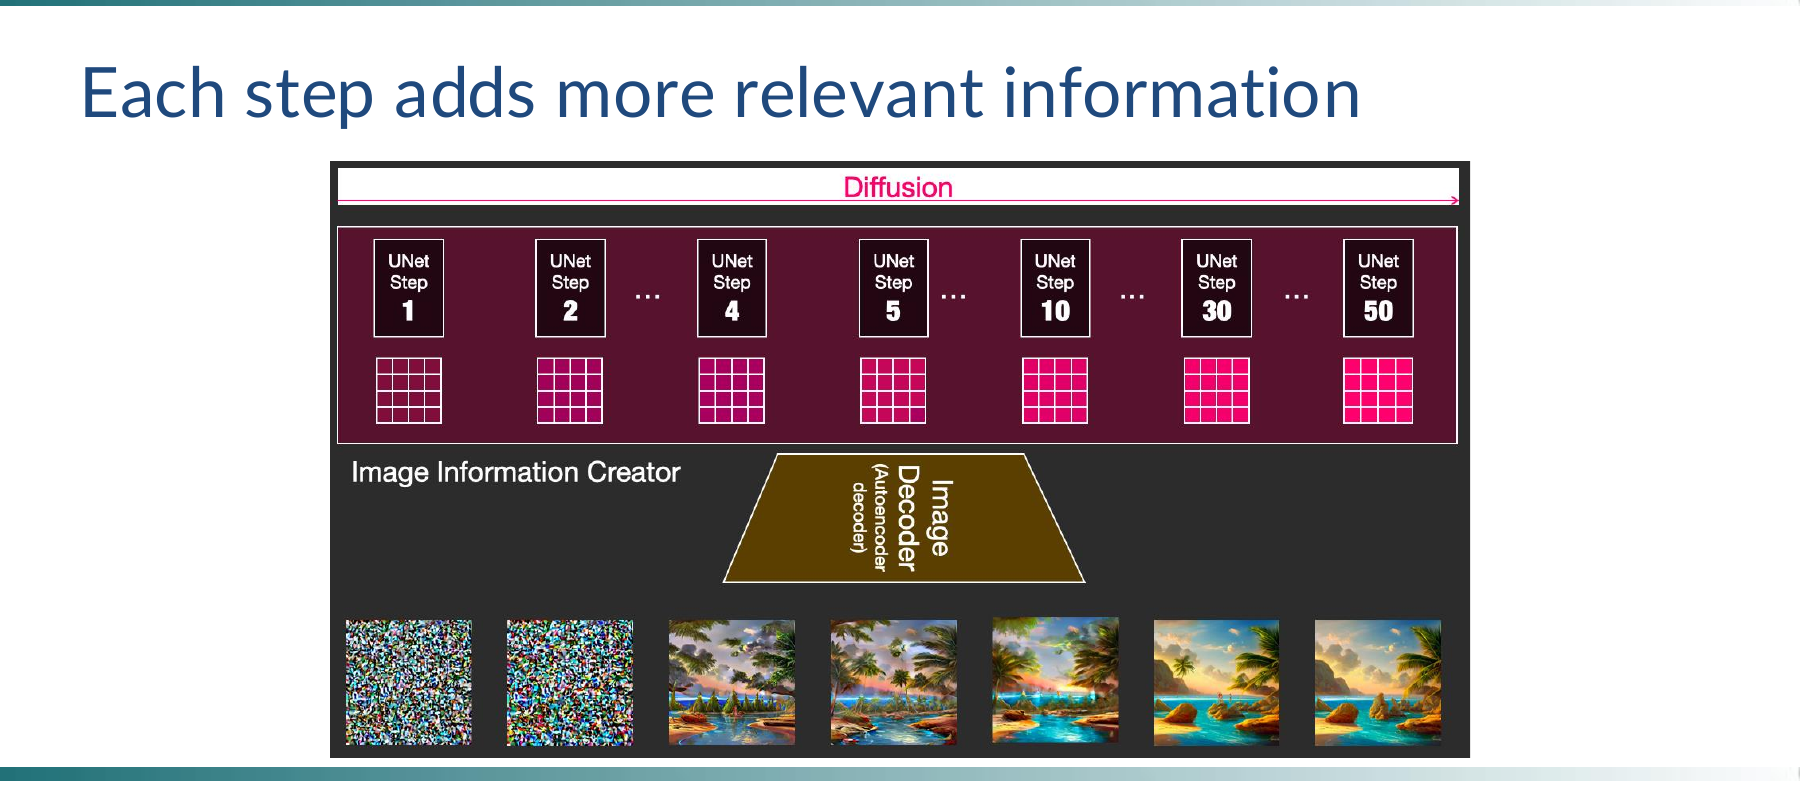
\includegraphics[width=0.90\linewidth]{figures/cf13_reverse_diffusion_steps.png}
  \caption{Processo di diffusione inversa. Partendo da un tensore
           di rumore puro (in basso a sinistra), il predittore del
           rumore (UNet) sottrae iterativamente il rumore stimato.
           A ogni passo si ottiene un'immagine via via più pulita,
           fino all'immagine finale generata (in basso a destra).}
  \label{fig:reverse_diffusion}
\end{figure}

\subsection{Noise Schedule}
\label{subsec:noise-schedule}

Il passaggio dall'immagine rumorosa a quella pulita avviene attraverso
una progressione definita dal \textbf{noise schedule}. Il noise schedule
specifica la quantità attesa di rumore residuo a ciascun passo di
campionamento e può essere configurato liberamente:

\begin{itemize}
  \item Si può scegliere di rimuovere la stessa quantità di rumore
        a ogni passo (\emph{uniform schedule}).
  \item Si può rimuovere più rumore nelle fasi iniziali del processo
        (\emph{decaying schedule}).
\end{itemize}

In ciascun passo il \textbf{sampler} sottrae esattamente la quantità
di rumore necessaria per raggiungere il livello atteso dal noise schedule
al passo successivo.

%------------------------------------------------------------
\section{Latent Diffusion: Diffusione nello Spazio Compresso}
\label{sec:latent-diffusion}

\subsection{Motivazione: Limiti della Diffusione nello Spazio dei Pixel}
\label{subsec:pixel-space-limits}

L'esecuzione del processo di diffusione direttamente nello \textbf{spazio
dei pixel} presenta limitazioni computazionali severe. Un'immagine
$512 \times 512$ con tre canali colore (rosso, verde, blu) occupa uno
spazio di $786\,432$ dimensioni: per ogni immagine è necessario
specificare quel numero di valori. Modelli come \textbf{Google Imagen}
e \textbf{OpenAI DALL-E} operano nello spazio dei pixel e, pur
adottando alcune ottimizzazioni, rimangono computazionalmente costosi e
non eseguibili su una singola GPU di consumo.

\subsection{Spazio Latente e Variational Autoencoder}
\label{subsec:latent-space-vae}

Stable Diffusion risolve questo problema spostando l'intero processo di
diffusione in uno \textbf{spazio latente} compresso, 48 volte più piccolo
dello spazio dei pixel. Questo approccio è reso possibile dalla
\textbf{manifold hypothesis}: le immagini naturali non sono casuali,
ma presentano un'alta regolarità strutturale (un viso segue specifiche
relazioni spaziali tra occhi, naso, guance e bocca; un cane ha quattro
zampe e una forma caratteristica). L'alta dimensionalità dello spazio
dei pixel è quindi in larga misura \emph{artificiale}: le immagini
naturali possono essere compresse nello spazio latente senza perdita
significativa di informazione \citep{bishop2024}.

La compressione e la successiva ricostruzione sono delegate a un
\textbf{Variational Autoencoder} (VAE), composto da:

\begin{description}
  \item[Encoder] Comprime l'immagine dallo spazio dei pixel
        $(3, 512, 512)$ alla rappresentazione latente $(4, 64, 64)$.
  \item[Decoder] Ricostruisce l'immagine dalla rappresentazione latente
        allo spazio dei pixel.
\end{description}

\begin{figure}[H]
  \centering
  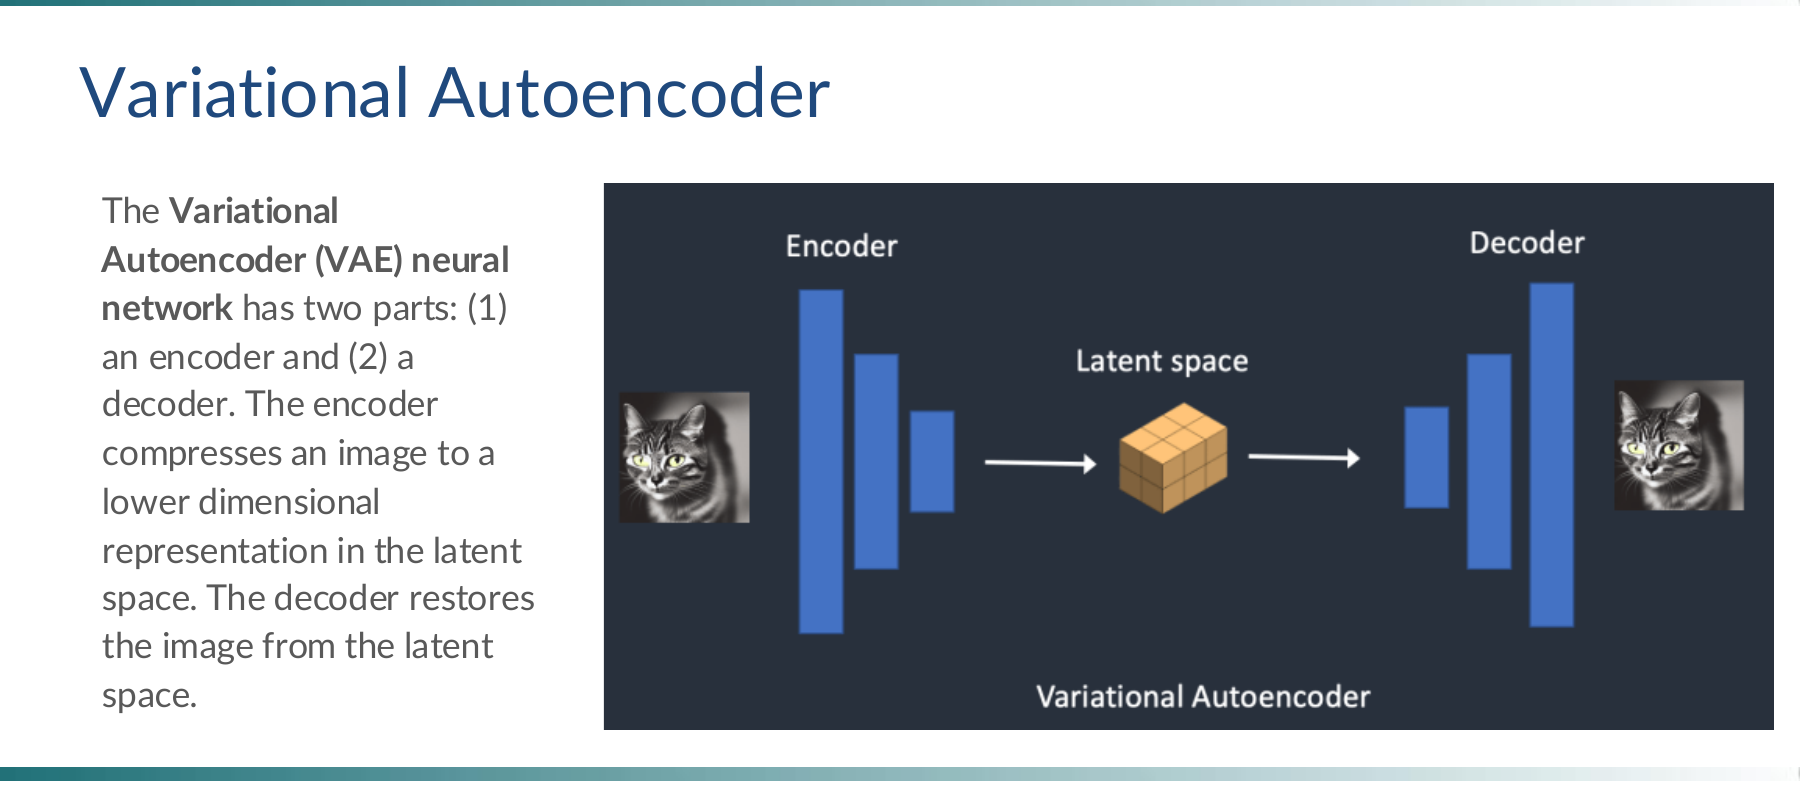
\includegraphics[width=0.88\linewidth]{figures/cf13_vae.png}
  \caption{Variational Autoencoder (VAE) utilizzato in Stable Diffusion.
           L'\emph{encoder} comprime l'immagine nello spazio latente
           $(4\times64\times64)$; il \emph{decoder} la ricostruisce
           nello spazio dei pixel $(3\times512\times512)$.}
  \label{fig:vae}
\end{figure}

\subsection{Addestramento e Inferenza Latente}
\label{subsec:latent-training-inference}

Durante l'\textbf{addestramento}, il processo di diffusione in avanti
opera direttamente sulle rappresentazioni latenti:

\begin{enumerate}
  \item L'immagine originale viene codificata nell'encoder VAE, ottenendo
        il corrispondente tensore latente.
  \item Vengono generati esempi di addestramento aggiungendo quantità
        variabili di rumore al tensore latente (non all'immagine pixel).
  \item Il Noise Predictor (UNet) viene addestrato a predire il rumore
        aggiunto nella rappresentazione latente.
\end{enumerate}

Durante l'\textbf{inferenza} (generazione), la diffusione inversa viene
eseguita interamente nello spazio latente:

\begin{enumerate}
  \item Si genera un tensore latente casuale.
  \item Il Noise Predictor stima il rumore del tensore latente.
  \item Il rumore stimato viene sottratto dal tensore latente.
  \item I passi 2 e 3 vengono ripetuti per il numero di passi di
        campionamento prescelti.
  \item Il decoder VAE converte il tensore latente finale nell'immagine
        generata.
\end{enumerate}

\paragraph{Nota sulla risoluzione.} La dimensione del tensore latente
è direttamente proporzionale alla risoluzione dell'immagine: per
immagini $512\times512$ il latente è $4\times64\times64$, mentre per
un'immagine ritratto $768\times512$ è $4\times96\times64$. Poiché
Stable Diffusion v1 è stato ottimizzato su immagini $512\times512$,
generare immagini di dimensioni superiori può produrre artefatti
(ad esempio oggetti duplicati).

%------------------------------------------------------------
\section{Condizionamento Testuale}
\label{sec:text-conditioning}

\subsection{Dalla Diffusione Non Condizionata al Condizionamento}
\label{subsec:conditioning-intro}

Il processo di diffusione inversa descritto finora è \textbf{non
condizionato}: il modello genera immagini casuali senza possibilità
di controllo sul contenuto. Per ottenere un modello \emph{text-to-image}
è necessario introdurre il \textbf{condizionamento}, ossia un meccanismo
che guidi il predittore del rumore affinché le immagini generate siano
coerenti con il prompt testuale.

\subsection{Text Encoder: CLIP}
\label{subsec:clip}

La componente di codifica testuale di Stable Diffusion è basata su
\textbf{CLIP} (\emph{Contrastive Language–Image Pre-training}), un
modello pre-addestrato su 400 milioni di coppie immagine--didascalia
raccolte dal Web (tramite i tag \texttt{alt} delle immagini).

CLIP è composto da due encoder:
\begin{description}
  \item[Image Encoder] Mappa immagini in uno spazio di embedding.
  \item[Text Encoder] Mappa testi nello stesso spazio di embedding.
\end{description}

L'addestramento avviene per \textbf{contrasto}: dato un mini-batch di
coppie (immagine, didascalia), CLIP massimizza la \emph{cosine
similarity} tra gli embedding di coppie corrispondenti e la minimizza
tra coppie non corrispondenti. Al termine dell'addestramento, embedding
di immagini e testi semanticamente simili si trovano in regioni vicine
dello spazio.

Il prompt testuale viene elaborato come segue:
\begin{enumerate}
  \item Un \textbf{tokenizer} converte ogni parola del prompt in un
        token numerico (ad esempio: ``photo'' $\to$ 50, ``cat'' $\to$
        239).
  \item Ogni token viene convertito in un vettore di embedding a 768
        valori.
  \item Gli embedding vengono processati dal \textbf{text transformer},
        che produce la sequenza finale di 77 vettori pronti per essere
        consumati dal Noise Predictor.
\end{enumerate}

\paragraph{Importanza della scelta del language model.} Il paper di
Google Imagen ha dimostrato sperimentalmente che la qualità del
modello linguistico utilizzato come encoder testuale ha un impatto
maggiore sulla qualità delle immagini generate rispetto alla dimensione
dei componenti di generazione dell'immagine. Per questo motivo Stable
Diffusion v2 ha adottato \textbf{OpenCLIP}, una variante open-source
di CLIP con modelli testuali fino a 354M parametri (contro i 63M di
CLIPText usato in v1), migliorando la qualità delle immagini generate.

\subsection{Cross-Attention: Integrazione del Testo nella UNet}
\label{subsec:cross-attention}

Il condizionamento testuale viene integrato nel Noise Predictor attraverso
un meccanismo di \textbf{cross-attention} inserito tra i blocchi ResNet
della UNet. I blocchi ResNet non accedono direttamente al testo:
i layer di cross-attention fondono le rappresentazioni testuali nello
spazio latente, consentendo ai blocchi ResNet successivi di sfruttare
tale informazione nel proprio processing.

Il \textbf{meccanismo di cross-attention} è un'estensione dell'attenzione
del Transformer che combina due sequenze di embedding distinte. A
differenza della \emph{self-attention}, che opera su una singola
sequenza, la cross-attention riceve:

\begin{itemize}
  \item Una sequenza $S_1$ (il condizionamento, ad esempio gli embedding
        testuali), da cui si derivano le matrici \textbf{Key} ($K$) e
        \textbf{Value} ($V$).
  \item Una sequenza $S_2$ (lo stato latente corrente), da cui si derivano
        le \textbf{Query} ($Q$).
\end{itemize}

Il calcolo segue la formula standard dell'attenzione scalata:
\begin{equation}
  \mathrm{CrossAttention}(S_1, S_2)
  \;=\;
  \mathrm{softmax}\!\left(
    \frac{(W_Q S_2)(W_K S_1)^\top}{\sqrt{d_k}}
  \right) W_V S_1
  \label{eq:cross-attention}
\end{equation}
dove $W_Q$, $W_K$, $W_V$ sono matrici di proiezione apprese, e $d_k$
è la dimensione delle chiavi. L'output ha la stessa dimensione e lunghezza
della sequenza $S_2$ (lo stato latente).

\begin{figure}[H]
  \centering
  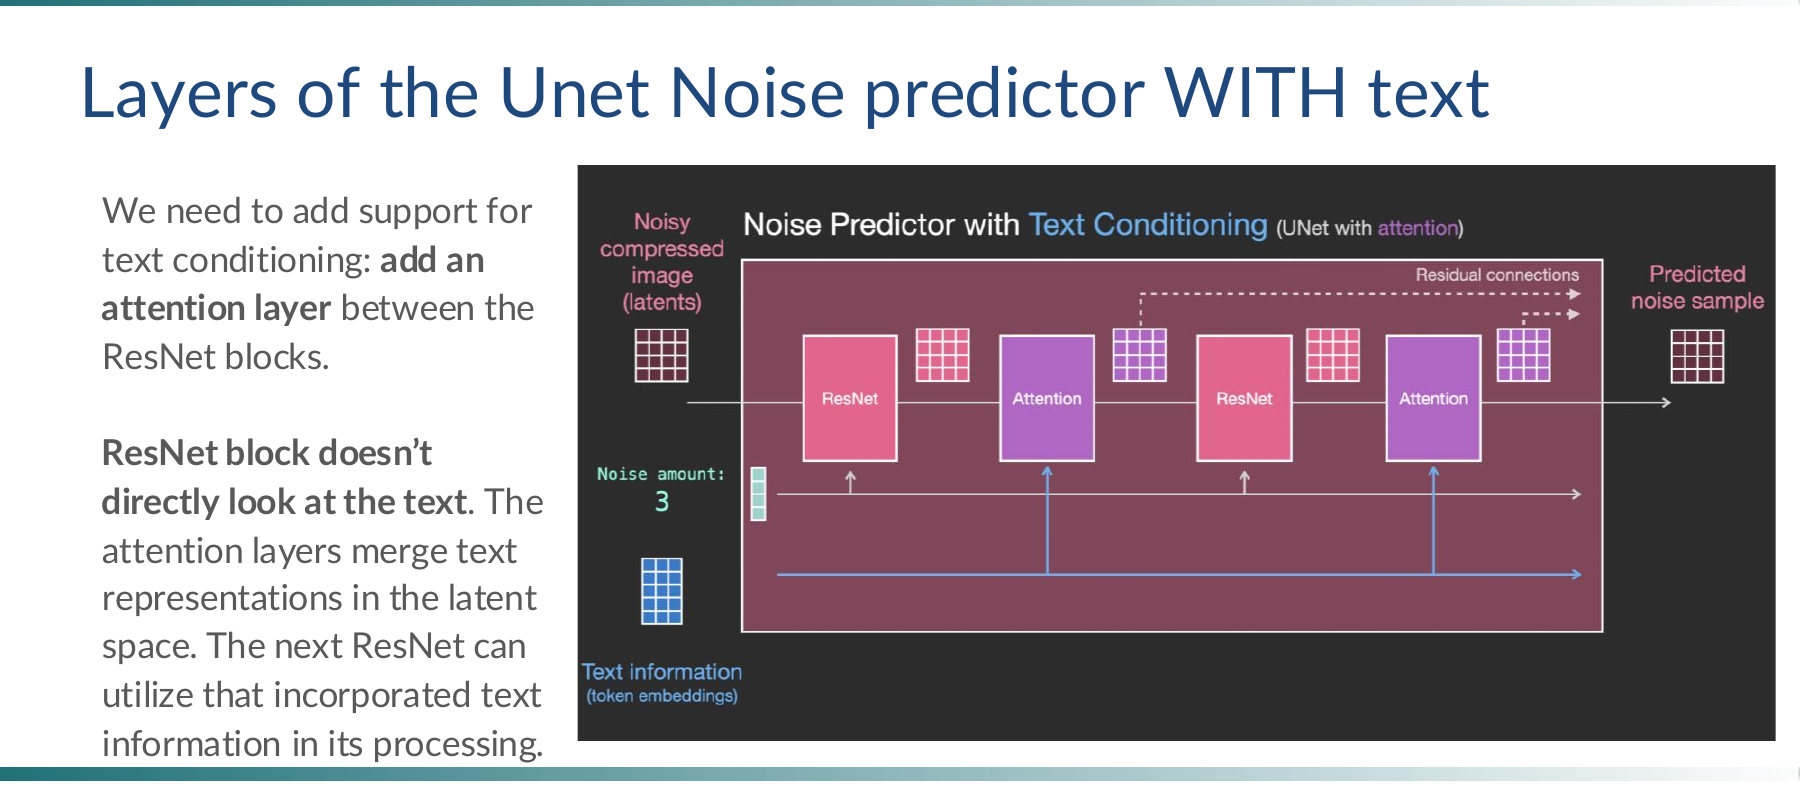
\includegraphics[width=0.88\linewidth]{figures/cf13_unet_with_attention.png}
  \caption{Struttura interna del Noise Predictor (UNet) con
           condizionamento testuale. I blocchi \emph{ResNet} processano
           il tensore latente; i layer di \emph{Attention} fondono
           la rappresentazione testuale nello spazio latente tramite
           cross-attention. Le connessioni residuali collegano le
           rappresentazioni intermedie alle parti più profonde della rete.}
  \label{fig:unet_attention}
\end{figure}

\begin{figure}[H]
  \centering
  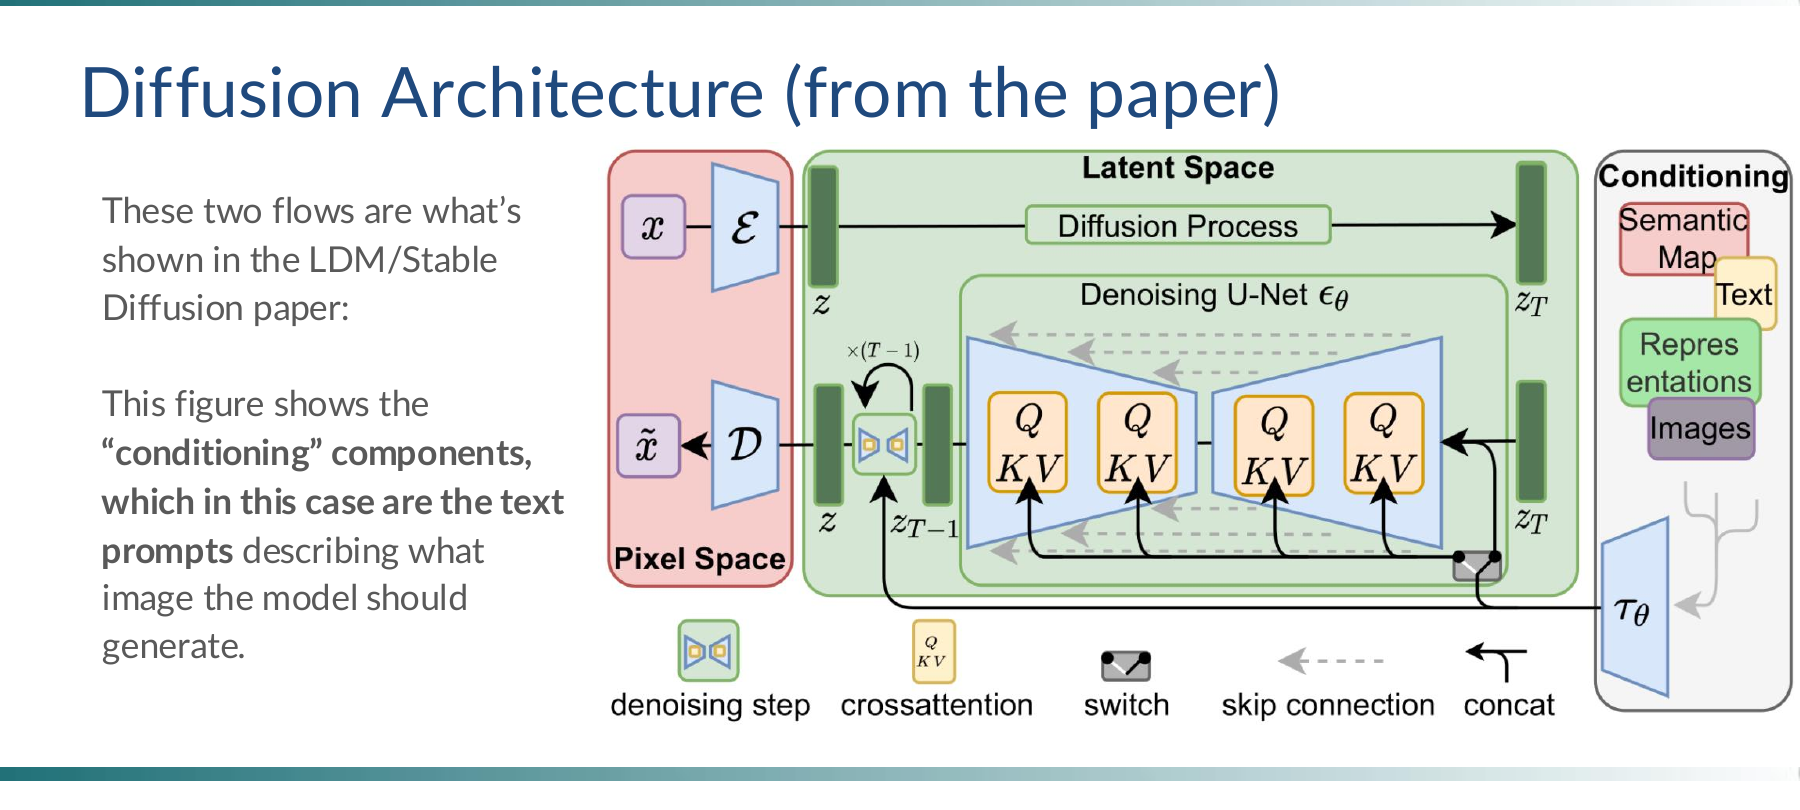
\includegraphics[width=0.92\linewidth]{figures/cf13_ldm_architecture.png}
  \caption{Architettura del Latent Diffusion Model (LDM) dal paper originale.
           L'encoder $\mathcal{E}$ comprime l'immagine nello spazio latente;
           la denoising UNet $\epsilon_\theta$ opera su tale spazio attraverso
           moduli di cross-attention ($Q$/$K$/$V$) che integrano il
           condizionamento $\tau_\theta$ (testo, mappe semantiche, immagini);
           il decoder $\mathcal{D}$ ricostruisce l'immagine nello spazio pixel.}
  \label{fig:ldm_architecture}
\end{figure}

\paragraph{Esempio: self-attention e cross-attention nel prompt.}
Considerando il prompt ``A man with blue eyes'': Stable Diffusion
sfrutta la \emph{self-attention} all'interno del prompt per associare
i token ``blue'' ed ``eyes'', generando un uomo con gli occhi blu e
non una camicia blu. Successivamente, la \emph{cross-attention} tra
prompt e immagine guida il processo di diffusione inversa verso immagini
contenenti occhi blu.

%------------------------------------------------------------
\section{Classifier-Free Guidance (CFG)}
\label{sec:cfg}

\subsection{Classifier Guidance}
\label{subsec:classifier-guidance}

Il \textbf{classifier guidance} è una tecnica che incorpora etichette
di classe nel processo di diffusione, guidando la generazione verso
immagini appartenenti a una categoria specifica (ad esempio ``gatto'').
La \emph{classifier guidance scale} controlla quanto strettamente il
processo di diffusione deve seguire l'etichetta:
\begin{itemize}
  \item Con una scala \textbf{bassa}, i campioni generati coprono
        un'ampia porzione della distribuzione della categoria.
  \item Con una scala \textbf{alta}, i campioni sono fortemente
        vincolati alle caratteristiche più tipiche e non ambigue della
        categoria, a scapito della diversità.
\end{itemize}

\subsection{Classifier-Free Guidance}
\label{subsec:cfg}

Sebbene il classifier guidance abbia ottenuto risultati eccellenti,
richiede un modello classificatore separato, il che complica
l'addestramento. Il \textbf{Classifier-Free Guidance} (CFG) risolve
questo problema incorporando la guida direttamente nel Noise Predictor,
senza la necessità di un classificatore esterno. Invece di etichette
di classe, il condizionamento avviene tramite \textbf{didascalie
testuali} e un modello di diffusione condizionato, esattamente come
nel paradigma text-to-image.

La \textbf{CFG scale} è il parametro che controlla l'intensità del
condizionamento:
\begin{itemize}
  \item Con CFG scale pari a \textbf{0}, la generazione è non
        condizionata (il prompt viene ignorato).
  \item Con valori \textbf{crescenti}, il processo di diffusione
        viene guidato sempre più strettamente verso il prompt testuale,
        producendo immagini più fedeli ma meno variate.
\end{itemize}

%------------------------------------------------------------
\section{Modalità di Generazione Avanzate}
\label{sec:advanced-modes}

\subsection{Image-to-Image}
\label{subsec:img2img}

Il metodo \textbf{image-to-image} (\emph{SDEdit}) estende la generazione
text-to-image ricevendo in input sia un prompt testuale sia un'immagine
di riferimento. L'immagine generata è condizionata da entrambi gli input.
Il processo si articola come segue:

\begin{enumerate}
  \item L'immagine di input viene codificata nello spazio latente
        tramite l'encoder VAE.
  \item Viene aggiunto rumore al tensore latente. Il parametro
        \textbf{denoising strength} controlla la quantità di rumore:
        con 0 non viene aggiunto rumore, con 1 viene aggiunto il
        massimo (il tensore diventa completamente casuale).
  \item Il Noise Predictor (UNet) riceve il tensore latente rumoroso
        e il prompt testuale, e predice il rumore nello spazio latente.
  \item Il rumore predetto viene sottratto dal tensore latente.
  \item I passi 3 e 4 vengono ripetuti per il numero prefissato di
        passi di campionamento.
  \item Il decoder VAE converte il tensore latente finale nell'immagine
        generata.
\end{enumerate}

\subsection{Inpainting}
\label{subsec:inpainting}

L'\textbf{inpainting} è un caso particolare di image-to-image in cui
il rumore viene aggiunto esclusivamente alle regioni dell'immagine che
si intende modificare. La quantità di rumore è controllata, anche in
questo caso, dal parametro di \emph{denoising strength}.

\subsection{Depth-to-Image}
\label{subsec:depth2img}

Il metodo \textbf{depth-to-image} estende l'image-to-image con un
condizionamento aggiuntivo basato su una \textbf{mappa di profondità}.
La mappa viene stimata automaticamente dall'immagine di input tramite
il modello \textbf{MiDaS} e viene fornita come ulteriore condizionamento
al Noise Predictor nella fase di predizione del rumore.

\subsection{Altri Condizionamenti: ControlNet}
\label{subsec:controlnet}

Il prompt testuale non è l'unico modo per condizionare un modello di
diffusione. \textbf{ControlNet} condiziona il Noise Predictor con
contorni rilevati automaticamente, pose umane stimate, mappe di
segmentazione e altri segnali strutturali, ottenendo un controllo
preciso sulla composizione delle immagini generate.

%------------------------------------------------------------
\section{Stable Diffusion v1 vs.\ v2}
\label{sec:sd-v1-v2}

\subsection{Differenze nel Modello}
\label{subsec:v1v2-model}

La principale differenza architetturale tra le due versioni riguarda
il \textbf{text encoder}:

\begin{itemize}
  \item \textbf{Stable Diffusion v1} utilizza \textbf{CLIP ViT-L/14}
        di OpenAI (63M parametri).
  \item \textbf{Stable Diffusion v2} utilizza \textbf{OpenCLIP},
        una variante open-source con modelli testuali fino a
        354M parametri (circa 5 volte più grande).
\end{itemize}

Il passaggio a OpenCLIP migliora la qualità delle immagini (modelli
linguistici più grandi migliorano le prestazioni generative) e offre
maggiore trasparenza al mondo della ricerca, poiché il training data
è pubblicamente documentato.

\subsection{Differenze nei Dati di Addestramento}
\label{subsec:v1v2-data}

\paragraph{Stable Diffusion v1.4} è stato addestrato su:
\begin{itemize}
  \item 237k passi a risoluzione $256\times256$ sul dataset
        \texttt{laion2B-en}.
  \item 194k passi a risoluzione $512\times512$ su
        \texttt{laion-high-resolution}.
  \item 225k passi a $512\times512$ su \texttt{laion-aesthetics v2 5+},
        con il 10\% di \emph{dropping} del condizionamento testuale.
\end{itemize}

\paragraph{Stable Diffusion v2.0} è stato addestrato su un sottoinsieme
di \texttt{LAION-5B} filtrato per contenuti espliciti (con classificatore
LAION-NSFW, $p_\text{unsafe}=0.1$, score estetico $\geq 4.5$):
\begin{itemize}
  \item 550k passi a $256\times256$.
  \item 850k passi a $512\times512$ su immagini con risoluzione
        $\geq 512\times512$.
  \item 150k passi con un \emph{v-objective}.
  \item 140k passi aggiuntivi a $768\times768$.
\end{itemize}

\paragraph{Stable Diffusion v2.1} è un fine-tuning di v2.0:
\begin{itemize}
  \item 55k passi aggiuntivi con $p_\text{unsafe}=0.1$.
  \item 155k passi con $p_\text{unsafe}=0.98$ (filtro NSFW
        sostanzialmente disattivato nelle ultime fasi).
\end{itemize}

\subsection{Differenze nelle Prestazioni}
\label{subsec:v1v2-perf}

Gli utenti riscontrano in v2 una minore capacità di controllare lo stile
artistico e di riprodurre celebrity rispetto a v1. Questo è probabilmente
dovuto alla differenza nei dati di addestramento: il dataset proprietario
di OpenAI su cui è stato addestrato CLIP ViT-L/14 contiene verosimilmente
più opere d'arte e fotografie di personaggi noti.

%------------------------------------------------------------
\section{Confronto con le GAN e con altri Modelli Generativi}
\label{sec:diffusion-vs-gans}

I modelli di diffusione hanno in larga misura superato le GAN in termini
di qualità generativa, in particolare per:

\begin{itemize}
  \item \textbf{Diversità dei campioni}: assenza del mode collapse,
        tipico delle GAN.
  \item \textbf{Stabilità dell'addestramento}: il processo di
        addestramento basato su una semplice loss di predizione del
        rumore è molto più stabile rispetto al gioco adversariale.
  \item \textbf{Qualità delle immagini}: campioni ad alta fedeltà
        con struttura semantica coerente, grazie al condizionamento
        testuale tramite cross-attention.
\end{itemize}

Il principale svantaggio rimane la \textbf{lentezza dell'inferenza}:
la generazione richiede decine o centinaia di passi di denoising, mentre
una GAN genera un campione in un singolo passaggio forward.

\begin{table}[H]
  \centering
  \caption{Confronto tra modelli generativi principali.}
  \label{tab:diffusion-comparison}
  \small
  \begin{tabular}{lllll}
    \toprule
    \textbf{Modello} & \textbf{Spazio di lavoro}
      & \textbf{Qualità} & \textbf{Diversità} & \textbf{Criticità} \\
    \midrule
    GAN
      & Pixel / latente
      & Alta
      & Bassa (mode collapse)
      & Instabilità, mode collapse \\
    VAE
      & Latente
      & Media
      & Alta
      & Campioni sfocati \\
    Normalizing Flow
      & Biiezione
      & Alta
      & Alta
      & Architettura vincolata \\
    Diffusion (pixel)
      & Pixel
      & Molto alta
      & Alta
      & Inferenza molto lenta \\
    Latent Diffusion
      & Latente
      & Molto alta (SOTA)
      & Alta
      & Inferenza lenta \\
    \bottomrule
  \end{tabular}
\end{table}

\paragraph{Considerazioni pratiche.}
\begin{enumerate}
  \item Il parametro \textbf{steps} (numero di passi UNet) è il
        principale trade-off qualità/velocità: più passi producono
        immagini migliori ma tempi di generazione più lunghi.
  \item La \textbf{CFG scale} controlla il bilanciamento tra fedeltà
        al prompt e diversità: valori tipici sono nell'intervallo 7--12.
  \item Il parametro \textbf{denoising strength} in image-to-image
        determina quanto l'immagine di output si discosterà da quella
        di input.
  \item In Stable Diffusion v1, è consigliabile mantenere almeno un
        lato dell'immagine a 512 pixel e usare un \emph{AI upscaler}
        per risoluzioni superiori, per evitare artefatti dovuti alla
        fuori distribuzione.
  \item I \textbf{VAE files} (decoder fine-tunati) possono essere
        utilizzati in Stable Diffusion v1 per migliorare la resa di
        occhi e volti, poiché la compressione VAE comporta una perdita
        di dettagli fini che il decoder specializzato è in grado di
        recuperare.
\end{enumerate}
